




\chapter{Discussion and Future Works}

Although the De-Whitening Filter can attenuate low frequency noise and effectively increase low frequency signal resolution, it limits the maximum excitation signal that can be sent to Photon Calibrator. This is one of intrinsic disadvantages of the De-Whitening filter. In Fig.\ref{fig:injcap} we estimated how much dynamical range will be sacrificed. 

\begin{figure}[hbt!]
\centering
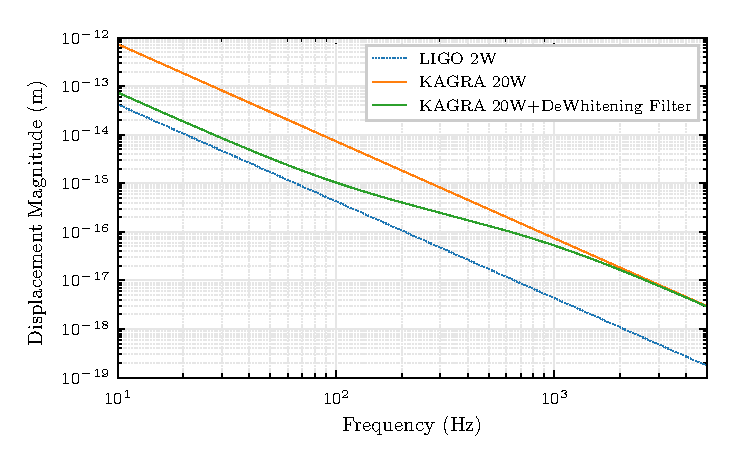
\includegraphics[width=0.8\textwidth]{figure/20WdeW}
\caption[Maximum Injection Capability]{Maximum Injection Capability. This is the maximum, assuming 100 percent optical efficiency, displacement of ETM could be generated by Photon Calibrator. It proportional to $1/f^2$ due to the force-to-displacement transfer function of suspended ETM. The green line indicate the maximum laser intensity modulation amplitude that is attenuated by De-Whitening filter.}
\label{fig:injcap}

\index{figures}
\end{figure}

For the quantization noise from DAC, one can adopt the so-called \emph{Noise Shaping} algorithm \cite{dac:shaping} to move the low frequency noise to the higher frequency regime, which will be removed by an anti-image filter before it comes into our PCal. Although it cannot increase the low frequency signal resolution that limited by DAC bit-depth, it dose not compromise maximum signal amplitude. As long as it is an approach independent approach to decrease the noise, we can apply it and De-Whitening filter at the same time if necessary.

On the other hand, naively, the noise problem can be solved by using a higher bit-depth DAC card. However, DACs with bit-depths higher than 16bits typically suffer from another noise source due to its \emph{Integral Nonlinearity}  (ref). Unless we dedicate significant resources into developing such high precision DAC chip and its auxiliary circuit, it might be challenging to find a satisfying commercial product at this moment. 

During the experiments, we found that carrying analog signals on 50m long D-sub cables may be problematic because we have such strict noise requirement. Installation of an extra digital control system near our PCal is favored.


We have successfully modulate PCal laser intensity according to several binary blak hole coalescence waveform templates. Once the main KAGRA interferometer start working, we can verify whether the ETM displacement has been generated as we expected. At the same time, will have ability to crosscheck the response of main interferometer, which is the main goal of hardware injection test. 





